\newpage
%\section{Results}
\chapter{Results}
\label{sec:results}
\section{Synthesis results}
All synthesis results in this chapter are synthesized for $PIXEL\_DATA\_WIDTH$ of 16, unless another value is especially mentioned. 
\subsection{Gauss-Jordan elimination}
\subsubsection{LUTs and registers}
\label{sec:synthesis:luts_and_registers_inverse}
Synthesis results for the first and the second implementation approach of the Gauss-Jordan elimination is shown in Figure \ref{fig:synthesis_result_naive_inverse}.

\begin{figure}[H]
\hbox{\hspace*{-2cm}                                                           

   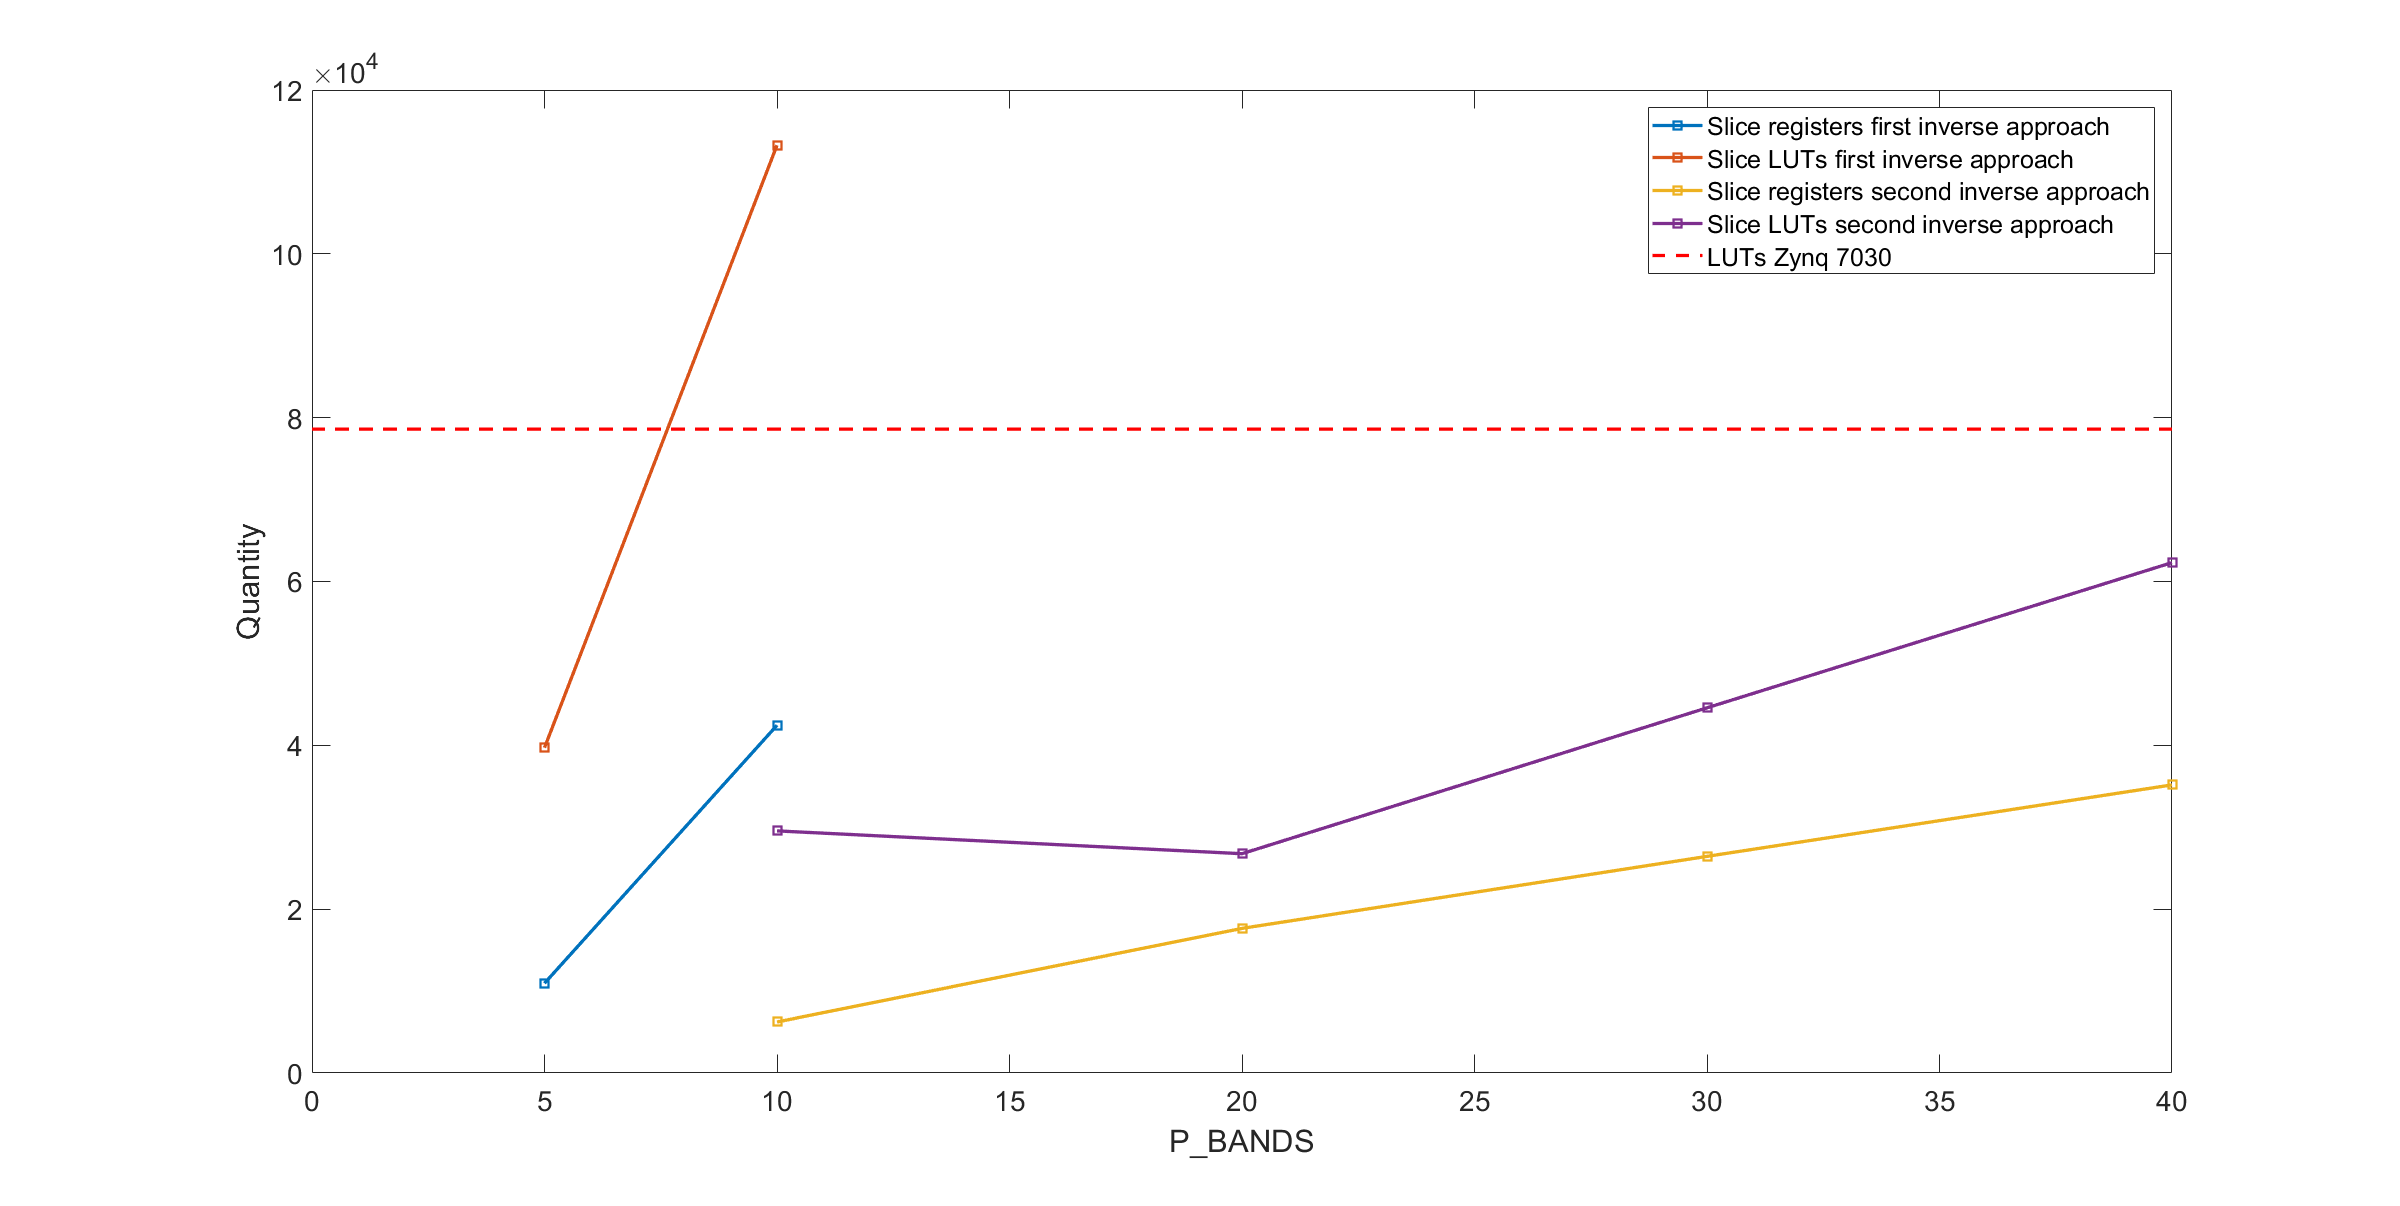
\includegraphics[scale=0.3]{images/inverse_hw/inverse_matrix_luts_and_registers.png}}
  \caption{Synthesis result for the first and second Gauss-Jordan implementation approach, showing number of LUTs and registers synthesized.  } 
  \label{fig:synthesis_result_naive_inverse}
\end{figure}